% This must be in the first 5 lines to tell arXiv to use pdfLaTeX, which is strongly recommended.
\pdfoutput=1
% In particular, the hyperref package requires pdfLaTeX in order to break URLs across lines.

\documentclass[11pt]{article}

% Remove the "review" option to generate the final version.
\usepackage[]{ACL2023}

% Standard package includes
\usepackage{times}
\usepackage{latexsym}

% For proper rendering and hyphenation of words containing Latin characters (including in bib files)
\usepackage[T1]{fontenc}
% For Vietnamese characters
% \usepackage[T5]{fontenc}
% See https://www.latex-project.org/help/documentation/encguide.pdf for other character sets

% This assumes your files are encoded as UTF8
\usepackage[utf8]{inputenc}

% This is not strictly necessary, and may be commented out.
% However, it will improve the layout of the manuscript,
% and will typically save some space.
\usepackage{microtype}

% This is also not strictly necessary, and may be commented out.
% However, it will improve the aesthetics of text in
% the typewriter font.
\usepackage{inconsolata}

\usepackage{graphicx}
\usepackage{xcolor}


% If the title and author information does not fit in the area allocated, uncomment the following
%
%\setlength\titlebox{<dim>}
%
% and set <dim> to something 5cm or larger.

\title{Extractive summarisation of biomedical research articles using TextRank, WordRank, and a hybrid approach}

% Author information can be set in various styles:
% For several authors from the same institution:
% \author{Author 1 \and ... \and Author n \\
%         Address line \\ ... \\ Address line}
% if the names do not fit well on one line use
%         Author 1 \\ {\bf Author 2} \\ ... \\ {\bf Author n} \\
% For authors from different institutions:
% \author{Author 1 \\ Address line \\  ... \\ Address line
%         \And  ... \And
%         Author n \\ Address line \\ ... \\ Address line}
% To start a seperate ``row'' of authors use \AND, as in
% \author{Author 1 \\ Address line \\  ... \\ Address line
%         \AND
%         Author 2 \\ Address line \\ ... \\ Address line \And
%         Author 3 \\ Address line \\ ... \\ Address line}

\author{Kristina Levina \\
  Linköping University, STIMA \\
  Course code: 732A81 \\
 \texttt{krile102} \\}

\begin{document}
\maketitle
\begin{abstract}
This project aims at offering a tool to generate a summary of a biomedical research manuscript automatically based on the main text. To this end, extractive summarisation is employed. The motivation behind choosing extractive summarisation is, in essense, the neccessety to preserve key sentences from the main text. Extractive summarisation will retrieve sentences based on their importance without rephrasing them, thereby excluding misinterpretations. The meaning preservation is crucial for scientific texts. In this project, PubMed dataset is used. A subset of 100 articles and their abstracts have been manually looked through and filtered so that articles and abstracts have similar characteristics in terms of relative number of sentences of the abstract to the main text. As a result, 24 articles and their human-written summaries (abstracts) were selected. Four algorithms were chosen for extractive summarisation: TextRank, WordRank, WordRank+TextRank, and BERSUM. Their performance was assessed using ROUGE (recall), BLEU (precision), and F1 score. The obtained results show that TextRank better than other algorithms suits for the considered task. 

\end{abstract}

\section{Introduction}

With increasing volume of published articles in medical research, it becomes increasingly difficult for doctors, medical staff, and public health officials to stay updated. Sometimes, a quick summary of an article can give sufficient information about whether a person wants to continue reading its full version. Not all texts have an abstract, and summarisation of such texts could assist the reader. Furthermore, sometimes the written abstract is too short and does not contain necessary information to decide upon reading the full article. Summarisation can assist in this case by generating a sufficiently large summary of the text. Ideally, the generated summary should have a well-defined structure, but this is beyond the scope of this project.

Summarisation techniques are classified into supervised and unsupervised  \citep{widyassari2019literature}. Supervised approaches require labeled datasets. The literature has reported examples of supervised text summarisation using AdaBoost and SVM classification \citep{widyassari2019literature}. Unsupervised models include TextRank \citep{mihalcea2004textrank} and K-means \citep{garcia2008text} among others.

Furthermore, summarisation techniques are classified into abstractive and extractive \citep{widyassari2019literature}. In extractive summarization, the text parts are extracted as a summary without modifications. In contrast, in abstractive summarization, a summary consists of new phrases or has words not present in the original text.

For summarisation of medical articles, extractive rather than abstractive summarisation is preferable. This is because it is crucial to preserve the content without modifications. Furthermore, as the labelled datasets are scarce in the literature, in this project, an unsupervised approach is chosen. Therefore, the objective of this project is to identify the best-performing tool for extractive summarisation of medical articles. The tested methods include TextRank, WordRank, WordRank+TextRank, and BERTSUM.

\section{Theory}
\subsection{PageRank}

The Google PageRank algorithm is explained in \citet{rogers2002google}. This algorithm allows to determine the importance of a web page. This is crucial for search engine optimisation. The PageRank of page $A$ is calculated as follows:

\begin{small}
\begin{equation}
 PR(A) = (1-d) + d \left(\frac{PR(T1)}{C(T1)} + ... + \frac{PR(Tn)}{C(Tn)}\right),
 \label{eq:pr}
\end{equation}
\end{small}
where $PR$ denotes PageRank; $d$ denotes a damping factor, which can be set between 0 and 1; pages $T1...Tn$ link to $A$; and $C(A)$ denotes the number of links going out of page $A$. The calculation is straightforward once $PR(T1)...PR(Tn)$ are known, but they are not. To exclude excessive influence of pages $T1..Tn$, the factor $d$ is set to 0.85 according to \citet{rogers2002google}. Terms $1-d$ are added so that $PR(A)$ is a probability distribution representing likelihood that a person randomly clicking on links will arrive at any particular page (sum of all pages' PageRanks will be one).

The recursive nature of Eq. (\ref{eq:pr}) means that one cannot determine $PR(A)$ without knowing $PR(T1)...PR(Tn)$. If a circular linking is introduced, this becomes cumbersome. However, initial parameters (PageRanks) can be set, and the calculation can be performed iteratively until convergence. This procedure can be computationally intensive if a large number of pages and links is involved. The resulting distribution would be close to the real probability distribution if not stacked in local minimum. Various optimisation techniques of PageRank algorithm have been proposed, including particle swarm optimisation (\citet{bastos2021inverse}).  An illustration of the PageRank algorithm is shown in Fig. \ref{fig:PR}.

\begin{figure}[!h]
\centering
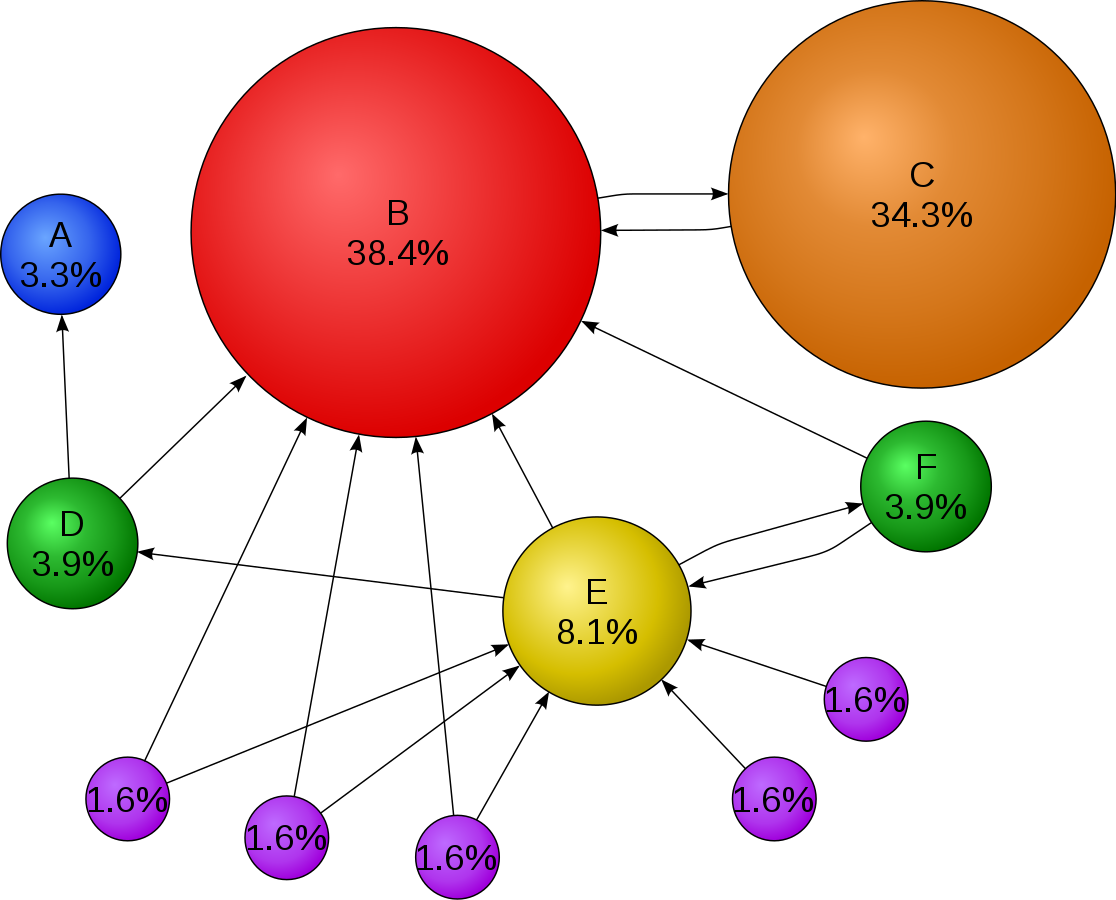
\includegraphics[scale = 0.175]{../figures/PR.png}
\caption{Figure source: \href{https://en.wikipedia.org/wiki/File:PageRanks-Example.svg}{Wikipedia}. Illustration of the PageRank algorithm. The percentage shows the perceived importance, and the arrows represent hyperlinks.\label{fig:PR}}
\end{figure}

\subsection{TextRank}
\label{subsect:textrank}

TextRank algorithm has been introduced by \citet{mihalcea2004textrank}. This is an unsupervised method of extractive summarisation. Sentences are ranked based on their similarity scores to each other. First, sentences are vectorised. Second, a similarity matrix between sentence vectors is computed. A graph is constructed such that sentences are nodes and similarity scores are edges. The PageRank algorithm is then run with sentences treated as pages and similarity scores as links. This simple idea enables to extract most important sentences (top ranked) from a text. The top sentence in the list will be that having the highest similarity to all other sentences in the text. In other words, the top extracted sentence will be related to most of other sentences in the text. A flowchart of WordRank is shown in Fig. \ref{fig:textrank}

\begin{figure}[!h]
\centering
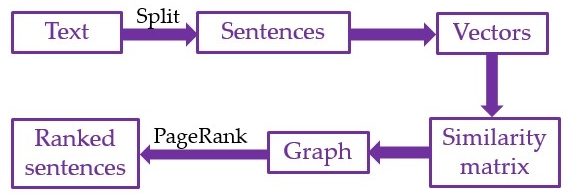
\includegraphics[scale = 0.5]{../figures/textrank.jpg}
\caption{Flowchart of TextRank.\label{fig:textrank}}
\end{figure}

\subsection{WordRank}
\label{subsect:wordrank}

WordRank is a modified version of TextRank \citep{reza2020}. The initial text is split into words. First, the words are vectorised. Second, a similarity matrix between word vectors is computed. A graph is constructed such that words are nodes and similarity scores are edges. The PageRank algorithm is then run with words treated as pages and similarity scores as links. Finally, the score of a sentence is the sum of the scores of all the words in that sentence. Top scored sentences are used for generating summary. A flowchart of WordRank is shown in Fig. \ref{fig:wordrank}

\begin{figure}[!h]
\centering
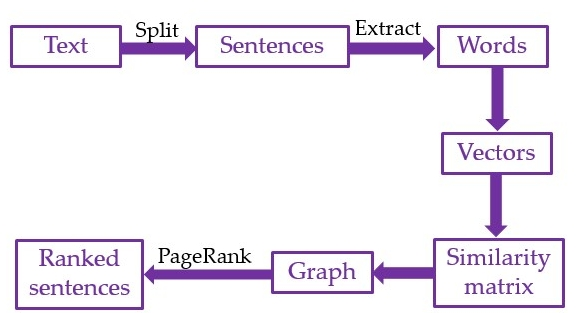
\includegraphics[scale = 0.5]{../figures/wordrank.jpg}
\caption{Flowchart of WordRank.\label{fig:wordrank}}
\end{figure}

\subsection{BERTSUM}

Bidirectional Encoder Representations from Transformers (BERT) is a family of masked-language models published in 2018 by Google \citep{devlin2019google}. The BERT architecture and operation principle is explained by \citet{rogers2021primer}. Citing them ``Fundamentally, BERT is a stack of Transformer encoder layers that consist of multiple self-attention “heads”. For every input token in a sequence, each head computes key, value, and query vectors, used to create a weighted representation. The outputs of all heads in the same layer are combined and run through a fully connected layer. Each layer is wrapped with a skip connection and followed by layer normalisation.''

The use of BERT for extractive summarisation is outlined by \citet{liu2019text}. The authors modified the BERT architecture (BERTSUM) for extractive text summarisation. Both architectures are shown in Fig. \ref{fig:bert}


\begin{figure*}[!h]
\centering
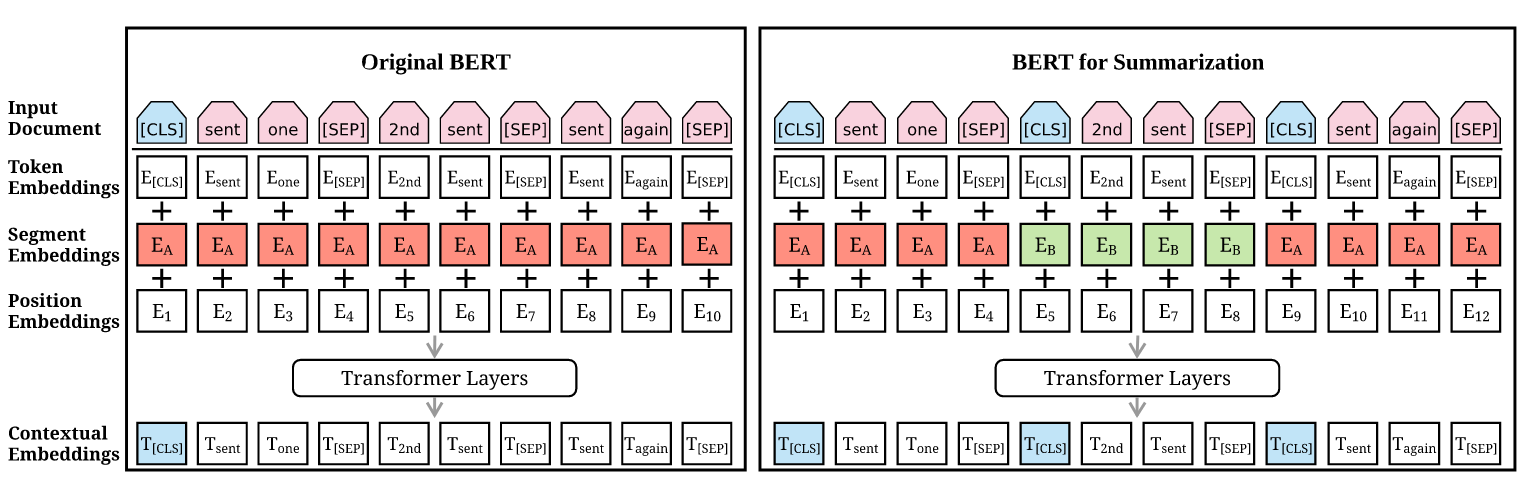
\includegraphics[scale = 0.35]{../figures/bert.png}
\caption{Figure source: \citet{liu2019text}.Architecture of the original BERT model (left) and BERTSUM (right). The input document is a sequence on top. It is followed by the summation of three types of embeddings for each token. The summed vectors are used
as input embeddings to several bidirectional Transformer layers, generating contextual vectors for each token. BERTSUM extends BERT by inserting multiple [CLS] symbols to learn sentence representations and using interval segmentation embeddings (illustrated in red and green color) to distinguish multiple sentences.\label{fig:bert}}
\end{figure*}


\subsection{Evaluation metrics}

How to compare human-generated summaries with machine-generated summaries? One can compare the occurrence of n-grams \citep{lin2003automatic} in both texts in terms of both precision and recall. In the context of comparison of a human-generated text with a machine-generated text, the recall metric is called ROUGE \citep{lin2003automatic}, and the precision metric is called BLEU \citep{papineni2002bleu}). 

ROUGE and BLEU are complementing evaluation metrics. If many n-grams from a machine-generated summary appear in a human-generated summary, BLEU is high, and if many n-grams from a human-generated summary appear in a machine-generated summary, ROUGE is high.

F1 score is a harmonic mean between ROUGE and BLEU:
\begin{equation}
 F1 = \frac{2\cdot BLEU \cdot ROUGE}{BLEU + ROUGE},
 \label{eq:f1}
\end{equation}
being a good performance indication metric overall.

One has to be aware of brevity penalty, when calculating BLEU. Consider the following example of a machine generated summary: \begin{verbatim}the the the the\end{verbatim} and a human-generated summary: \begin{verbatim}the cat likes mice\end{verbatim} The BLEU metric will be $4/4 = 1$ (aka four words from the machine-generated summary appear in the human-generated summary). However, the machine-generated summary is poor. To fix this, a brevity penalty is introduced: the repetition number of a word to take into account in BLEU can be as high as the repetition number of the word in the human-generated summary. In the example above, \texttt{the} appears only once in the machine-generated summary. Thus, BLEU is $1/4=0.25$, reflecting the poor quality of the machine-generated summary.

\section{Data}
\label{sect:data}

Data are taken from the paper by \citet{cohan2018discourse}. This dataset contains a large collection (100,000) of scientific articles from the biomedical domain (OpenAccess PubMed articles). Data are hosted in \href{https://github.com/armancohan/long-summarization}{GitHub}. Each article has the following fields: 
\begin{verbatim}
{ 
  'article_id': str,
  'abstract_text': List[str],
  'article_text': List[str],
  'section_names': List[str],
  'sections': List[List[str]]
}
\end{verbatim}

For this project, I have looked through 100 articles and considered only articles meeting the following assumptions: First, the provided abstract should be between 8\%--12\% of the main text in terms of number of sentences. This is to ensure similar conditions for generating summaries. Second, the number of sentences of the main manuscript text should be larger than 50 to meet the objective of long document summarisation. Out of 100 articles, only 24 met this conditions.

An example of the beginning of one chosen article is as follows:

\texttt{'["anxiety affects quality of life in those living with parkinson \'s disease ( pd ) more so than overall cognitive status, motor deficits, apathy, and depression [ 13 ] .", \'although anxiety and depression are often related and coexist in pd patients, recent research suggests that anxiety rather than depression is the most prominent and prevalent mood disorder in pd [ 5, 6 ] . yet,\', }

The beginning of the corresponding summary is as follows:

\texttt{'["<S> research on the implications of anxiety in parkinson \'s disease ( pd ) has been neglected despite its prevalence in nearly 50\% of patients and its negative impact on quality of life . </S>", \'<S> previous reports have noted that neuropsychiatric symptoms impair cognitive performance in pd patients }

The data have been already tokenised. From the abstract text, <S> and </S> tags were removed. Further preprocessing included stop word removal, lemmatisation, and non-alphabetic characters' removal. This preprocessing has been done using the Spacy language model. Stop words were removed to avoid sentence ranking based on common and frequent words rather than important words. Lemmatisation was used to treat same words in an exactly same manner. Non-alphabetic characters were removed to avoid their influence on the ranking results. Punctuation and numerals should not affect the sentence importance.
 

\section{Method}

After data pre-processing explained in Sect. \ref{sect:data}, the initial text was split into a list of sentences (see function \texttt{preprocess} in the \texttt{main\_project.py} file). All the methods explained below yielded as many sentences as was in the corresponding human-written summary to ensure equal evaluation conditions.´                                                                                                                                        
                                                                                                                                          
\subsection{TextRank}

Following the procedure outlined in Sect. \ref{subsect:textrank}, a list of preprocessed sentences was input into \texttt{textrank} function (see \texttt{main\_project.py} file). Then the sentences were vectorised as bags of words using word embeddings from \texttt{Spacy}:

\begin{equation}
 vect(sent) = \sum_{i = 1}^N (embed(word_i)),
\end{equation}
where $word_i$ is a word of a sentence $sent$, $N$ is the number of all words in the sentence, and $embed(word_i)$ is the \texttt{Spacy} embedding of $word_i$.

The cosine similarity was then used to compute the similarity between the vectors of all sentences. The obtained similarity scores were used to construct a similarity matrix. The obtained similarity matrix was transformed into a graph using Python library \texttt{nx}. PageRank was run using \texttt{nx.pagerank}. The sorted sentence scores were outputted from the function \texttt{textrank}.

\subsection{WordRank}

Following the procedure outlined in Sect. \ref{subsect:wordrank}, a list of preprocessed sentences was input into \texttt{wordrank} function (see \texttt{main\_project.py} file). Herein, the words were embedded using \texttt{Spacy} embeddings. The cosine similarity was again used to compute similarity scores between word vectors. The obtained similarity scores were used to construct a similarity matrix. The obtained similarity matrix was transformed into a graph using Python library \texttt{nx}. PageRank was run using \texttt{nx.pagerank}. The sentence score was found as the summation of the scores of all words in the sentence. The sorted sentence scores were outputted from the function \texttt{textrank}.

\subsection{Hybrid}

The TextRank algorithm is bound to favour longer sentences, resulting in high BLEU score. In contrast, the WordRank algorithm favours sentences with the most related words to other words, resulting in high ROUGE. This idea is outlined by \citet{reza2020}. Could this two algorithms be combined so that the F1 score is higher than that of individual algorithms? \citet{reza2020} used a combination of WordRank and TextRank. First, WordRank was run to extract 64\% of the initial sentences. The TextRank was then run on these 64\% extracted sentences to obtain 8\% of the initial text as a generated summary. This combination worked best in \citet{reza2020}. 

Here, their experiment is repeated. In addition, a hybrid algorithm with WordRank extracting 80\% of the initial text and TextRank extracting the required number of sentences was run. The relevant code is found in functions \texttt{hybrid64} and \texttt{hybrid80} in the \texttt{main\_project.py} file.

\subsection{BERTSUM}

The BERTSUM was run on the preprocessed initial texts on Google Colab using the library \texttt{bert-extractive-summarizer}.

\subsection{Evaluation}

The human-written summaries and the machine-generated summaries were split into unigrams, bigrams, and trigrams. Subsequently, BLEU, ROUGE, and F1 scores were obtained. The brevity factor was taken into the account. (See function \texttt{evaluation\_report} in the \texttt{main\_project.py} file)

After all 24 experiments, the obtained BLEU, ROUGE, and F1 scores were averaged, and their mean (e.g. $\overline{F1}$) and standard deviation (e.g. $\sigma(F1)$) values were obtained. The corresponding margins of error (95\%confidence) were computed following the usual frequentist approach:

\begin{equation}
 F1 = \overline{F1} \pm 1.96 \frac{\sigma(F1)}{\sqrt(24)}.
\end{equation}


\section{Results}

The ROUGE\_1, BLEU\_1, and F1\_1 scores respectively denote ROUGE, BLEU, and F1 scores of unigrams between the human-written and generated summaries. The results are shown in Fig. \ref{fig:uni} and Tables \ref{tab:means} and \ref{tab:mors}. TextRank (36.0), Hybrid64 (35.7) and Hybrid80 (35.9) yield high mean F1\_1 scores relative to WordRank (30.3), but considering margin of error, the estimation by Hybrid80 is slightly more robust (35.9 $\pm$ 3.3 versus 36.0 $\pm$ 3.7). The highest mean F1\_1 score shows BERTSUM (37.7 $\pm$ 3.9). TextRank (27.0 $\pm$ 3.7), Hybrid64 (26.7 $\pm$ 3.1), and Hybrid80 (26.8 $\pm$ 3.2) yield high mean BLEU\_1 scores relative to WordRank (20.8 $\pm$ 3.2). The highest BLEU\_1 value shows BERTSUM (30.4 $\pm$ 3.7). WordRank yields the highest ROUGE\_1 score (60.1 $\pm$ 4.1) in comparison to other algorithms. The lowest ROUGE\_1 score belongs to BERTSUM (51.2 $\pm$ 5.0).

The ROUGE\_2, BLEU\_2, and F1\_2 scores respectively denote the ROUGE, BLEU, and F1 scores of bigrams between the human-written and generated summaries. The results are shown in Fig. \ref{fig:bi} and Tables \ref{tab:means} and \ref{tab:mors}. The ROUGE\_3, BLEU\_3, and F1\_3 scores respectively denote the ROUGE, BLEU, and F1 scores of trigrams between the human-written and generated summaries. The results are shown in Fig. \ref{fig:tri} and Tables \ref{tab:means} and \ref{tab:mors}. TextRank shows the highest values of ROUGE\_2 and ROUGE\_3 (21.2 $\pm$ 4.9 and 10 $\pm$ 3.7, respectively) and F1\_2 and F1\_3 (13.4 $\pm$ 3.2 and 6.5 $\pm$ 2.5, respectively). However, regarding BLEU\_2, BERTSUM (10.3 $\pm$ 2.9) yields slightly higher mean value than TextRank (10.1 $\pm$ 2.7). 

The total running times of all four algorithms for summarisation of 24 data samples is shown in Table \ref{tab:time}. TextRank (1 min) performs 16 times faster than WordRank, Hybrid64, and Hybrid80 algorithms (16 min). BERTSUM (24 min) runs very slowly in comparison to TextRank.

\begin{figure}[!h]
\centering
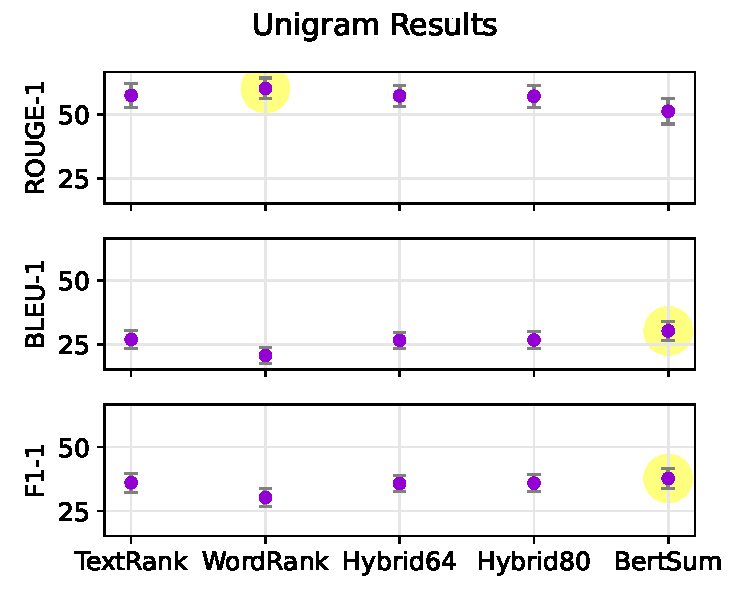
\includegraphics[scale = 0.5]{../figures/unigrams.pdf}
\caption{ROUGE, BLEU, and F1 score of unigrams between the human-written and generated summaries.\label{fig:uni}}
\end{figure}

\begin{figure}[!h]
\centering
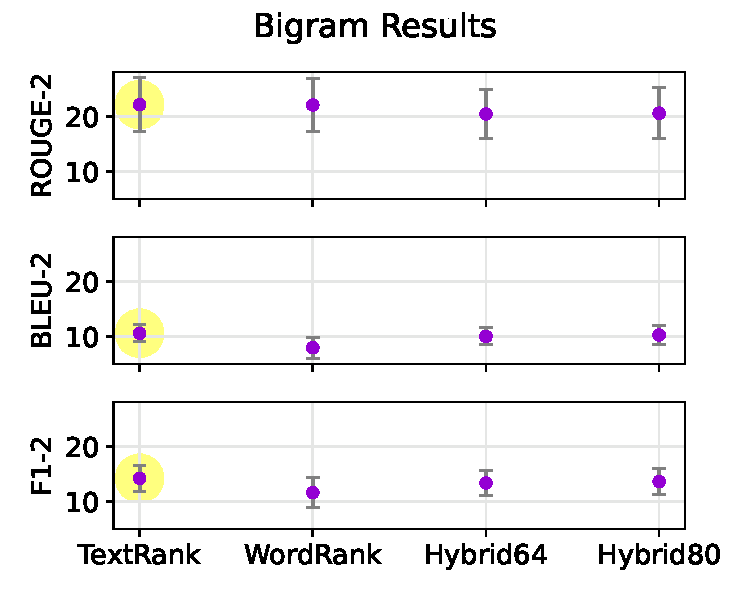
\includegraphics[scale = 0.5]{../figures/bigrams.pdf}
\caption{ROUGE, BLEU, and F1 score of bigrams between the human-written and generated summaries.\label{fig:bi}}
\end{figure}

\begin{figure}[!h]
\centering
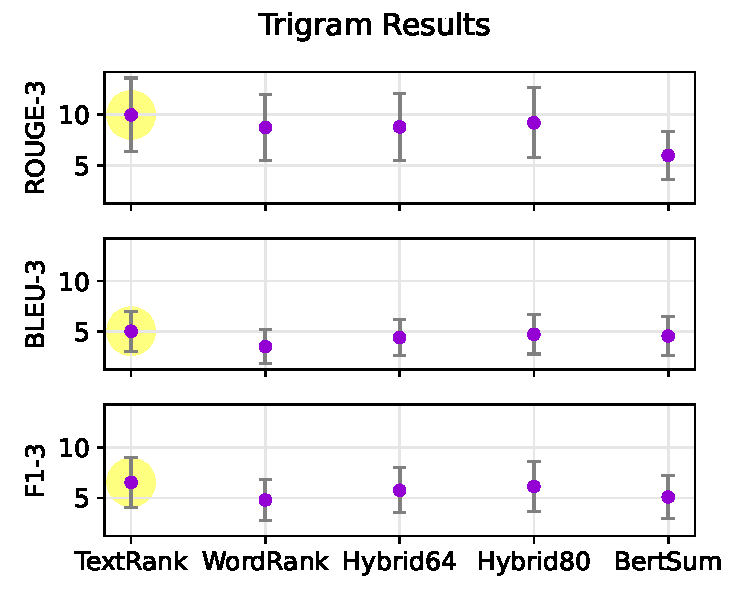
\includegraphics[scale = 0.5]{../figures/trigrams.pdf}
\caption{ROUGE, BLEU, and F1 score of trigrams between the human-written and generated summaries.\label{fig:tri}}
\end{figure}

\begin{table*}[!h]
\centering
\begin{tabular}{l|lllll}
\hline
&\textbf{TextRank} & \textbf{WordRank} & \textbf{Hybrid64} & \textbf{Hybrid80} & \textbf{BERTSUM}\\
\hline
ROUGE\_1 & 57.4 & \textbf{60.1} & 57.2 & 57.1& 51.2\\
ROUGE\_2 & \textbf{21.2} & 20.3 & 19.9 & 20.3& 16.0\\
ROUGE\_3 & \textbf{10.0} & 8.7 & 8.8 & 9.2& 6.0\\
BLEU\_1 & 27.0 & 20.8 & 26.7 & 26.8& \textbf{30.4}\\
BLEU\_2 & 10.1 & 7.3 & 9.5 & 9.8& \textbf{10.3}\\
BLEU\_3 & \textbf{5.0} & 3.5 & 4.4 & 4.7& 4.6\\
F1\_1 & 36.0 & 30.3 & 35.7 & 35.9& \textbf{37.7}\\
F1\_2 & \textbf{13.4} & 10.4 & 12.6 & 12.9& 12.3\\
F1\_3  & \textbf{6.5} & 4.8 & 5.8 & 6.1& 5.1\\
\hline
\end{tabular}

\caption{\label{tab:means}
Mean values of the ROUGE, BLEU, and F1 metrics for unigrams, bigrams, and trigrams yielded by TextRank, WordRank, Hybrid64, Hybrid80, and BERTSUM methods.
}
\end{table*}

\begin{table*}[!h]
\centering
\begin{tabular}{l|lllll}
\hline
&\textbf{TextRank} & \textbf{WordRank} & \textbf{Hybrid64} & \textbf{Hybrid80} & \textbf{BERTSUM}\\
\hline
ROUGE\_1 & 4.7 & 4.1 & 4.1 & 4.3 & 5.0\\
ROUGE\_2 & 4.9 & 4.6 & 4.4 & 4.7 & 4.0\\
ROUGE\_3 & 3.7 & 3.2 & 3.3 & 3.5 & 2.4\\
BLEU\_1 & 3.7 & 3.2 & 3.1 & 3.2 & 3.7\\
BLEU\_2 & 2.7 & 2.2 & 2.3 & 2.5 & 2.9\\
BLEU\_3 & 2.0 & 1.7 & 1.8 & 1.9 & 2.0\\
F1\_1 &  3.7 & 3.6 & 3.2 & 3.3 & 3.9\\
F1\_2 & 3.2 & 2.8 & 2.9 & 3.1 & 3.2\\
F1\_3  & 2.5 & 2.0 & 2.2 & 2.4 & 2.1\\
\hline
\end{tabular}
\caption{\label{tab:mors}
Margins of error values of the ROUGE, BLEU, and F1 metrics for unigrams, bigrams, and trigrams yielded by TextRank, WordRank, Hybrid64, Hybrid80, and BERTSUM methods.
}
\end{table*}


\begin{table*}[!h]
\centering
\begin{tabular}{l|lllll}
\hline
&\textbf{TextRank} & \textbf{WordRank} & \textbf{Hybrid64} & \textbf{Hybrid80} & \textbf{BERTSUM}\\
\hline
Running time (min) & 1 & 16 & 16 & 16 & 24\\
\hline
\end{tabular}
\caption{\label{tab:time}
Running time (min) of all five algorithms considered in this project.
}
\end{table*}

\subsection{Example result}

The human-written summary: "\textcolor{cyan}{Research on the implications of anxiety in parkinson's disease (pd) has been neglected} despite its prevalence in nearly 50\% of patients and its negative impact on quality of life. Previous reports have noted that neuropsychiatric symptoms impair cognitive performance in pd patients; \textcolor{cyan}{However, to date, no study has directly compared pd patients with and without anxiety to examine the impact of anxiety on cognitive impairments in pd}. \textcolor{gray}{This study compared cognitive performance across 50 pd participants with and without anxiety (17 pda+; 33 pda)}, who underwent neurological and neuropsychological assessment. Group performance was compared across the following cognitive domains: simple attention/visuomotor processing speed, executive function (e.g., set-shifting), working memory, language, and memory/new verbal learning. \textcolor{teal}{Results showed that pda+ performed significantly worse on the digit span forward and backward test and part b of the trail making task (tmt-b) compared to the pda group}. There were no group differences in verbal fluency, logical memory, or tmt-a performance. In conclusion, anxiety in pd has a measurable impact on working memory and attentional set-shifting."

The TextRank-generated summary: '\textcolor{teal}{More specifically, we found that pd patients with anxiety were more impaired on the trail making test part b which assessed attentional set-shifting, on both digit span tests which assessed working memory and attention, and to a lesser extent on the logical memory test which assessed memory and new verbal learning compared to pd patients without anxiety}. \textcolor{gray}{Taken together, thus, all participants who scored within a  depressed  (hads - d > 6) range were excluded from this study, in attempt to examine a refined sample of pd patients with and without anxiety in order to determine the independent effect of anxiety on cognition}. Future studies should perform diagnostic interviews with participants (e.g., using dsm - v criteria) rather than relying on self-reported measures to group participants, in order to better understand whether the type of anxiety disorder (e.g., social anxiety, phobias, panic disorders, and generalized anxiety) influences cognitive performance differently in pd. \textcolor{gray}{Given that research on healthy young adults suggests that anxiety reduces processing capacity and impairs processing efficiency, especially in the central executive and attentional systems of working memory [26, 27], we hypothesized that pd patients with anxiety would show impairments in attentional set-shifting and working memory compared to pd patients without anxiety}. \textcolor{cyan}{Considering many previous studies have investigated the influence of depression on cognition in pd without accounting for the presence of anxiety and the inconsistent findings reported to date}, we recommend that future research should try to disentangle the influence of anxiety versus depression on cognitive impairments in pd. Considering the growing number of clinical trials for treating depression, \textcolor{cyan}{there are few if any for the treatment of anxiety in pd. It is also striking that, to date, no study has examined the influence of anxiety on cognition in pd by directly comparing groups of pd patients with and without anxiety while excluding depression}. For example, may disrupt compensatory processes in pd patients and explain the cognitive impairments specifically in working memory and attention seen in pd patients with anxiety.'

This example clearly shows that TextRank favours longer sentences. Does this example make sense? The study motivation (in cyan) is captured in the generated summary. The study objective (in grey  is captured to some extent. Methods are been captured. Results (in teal) have been captured to some extent. Conclusion is been captured. I believe that the generated summary is okay but could be better.

\section{Discussion}

First, it should be emphasised that the running time of TextRank is superior. If a fast summarisation should be performed, TextRank generates the text fast with a good F1 score in comparison with other investigated algorithms. 

Confirming the discussion by \citet{reza2020}, TextRank favouring longer sentences results in higher BLEU than WordRank for unigrams, bigrams, and  trigrams. However, WordRank results in higher ROUGE than TextRank only for unigrams. TextRank starts to dominate WordRank in terms of the mean ROUGE values when assessing bigram and trigram co-occurrence.

The best-performing model is TextRank considering the low running time and the highest F1\_2 and F1\_3 scores. The F1\_1 score of TextRank (36.0) is within the margin of error of BERTSUM (37.7 $\pm$ 3.9). Thus, considering the long running time of BERTSUM, TextRank should be favoured for the task at hand.

Important result of the analysis is that combining WordRank with TextRank not necessarily yields better F1 scores than TextRank. However, this conclusion cannot be made because TextRank, Hybrid64, and Hybrid80 all yield similar results, considering their margins of error.

\subsection{Comparison with \citet{reza2020}}

\citet{reza2020} used the same dataset for extractive summarisation. However, their number of samples was 9,978 (it was 24 in this project). Furthermore, they obtained median F1 scores rather than mean F1 scores. Their results are as follows:
\begin{verbatim}
 WordRank: median(F1_1) = 35.56 and 
           SD(F1_1) = 0.1092 
 TextRank: median(F1_1) = 38.47 and 
           SD(F1_1) = 0.1085 
 Hybrid64: median(F1_1) = 38.28 and 
           SD(F1_1) = 0.1090 
 WordRank: median(F1_2) = 14.95 and 
           SD(F1_2) = 0.0825  
 TextRank: median(F1_2) = 16.56 and 
           SD(F1_2) = 0.0856 
 Hybrid64: median(F1_2) = 16.70 and 
           SD(F1_2) = 0.0862  
\end{verbatim}

Hence, the median F1 scores are higher for all algorithms than their means in this work. Perhaps, this is achieved by avoiding excessive influence of bad results, which median can do because it is robust to outliers. 

That is, for WordRank, their F1\_1 ($35.56$) is higher than $30.3 \pm 3.6$ including margin of error. For TextRank, their F1\_1 ($38.47$) is within the interval of $36.0 \pm 3.7$ (95\% confidence) obtained herein. For Hybrid64, their F1\_1 ($38.28$) is within the interval of $35.7 \pm 3.2$ (95\% confidence) obtained herein. 

Now, let us compare the results for bigram co-occurrence. For WordRank, their F1\_2 ($14.95$) is higher than $10.4 \pm 2.8$ including margin of error. For TextRank, their F1\_2 ($16.56$) is higher than $13.4 \pm 3.2$ including margin of error. For Hybrid64, their F1\_2 ($16.70$) is higher than $12.6 \pm 2.9$ including margin of error. 

However, comparing the best-performing models, TextRank yielded the highest median F1\_1 score ($38.47$) by \citet{reza2020}. In this project, BERTSUM yielded the highest mean F1\_1 score (37.7 $\pm$ 3.9). These results are similar, considering margin of error. For bigram co-occurrence, Hybrid64 yielded the highest median F1\_2 score ($16.70$) by \citet{reza2020}. In this project, TextRank yielded an F1\_2 score of $13.4 \pm 3.2$, being lower than 16.70 including margin of error.


\subsection{Limitations and future work}

The biggest limitation of this project is low amount of data. I believe that more data samples could be collected for assessment. In addition, articles meeting different conditions than those outlined in Sect. \ref{sect:data} could be collected. The obtained results could be compared. This remains future work.

Another limitation is absence of the inverse hybrid analysis: run TextRank first and WordRank second. This experiment should be conducted and remains future work.

The third limitation is absence of the analysis of the third variant of a hybrid model. BERTSUM yielded high BLEU scores when assessing unigram and bigram co-occurrence. Thus, BERTSUM could be combined with WordRank yielding high ROUGE values. This could compensate for the low ROUGE of BERTSUM and the low BLEU of WordRank. It would be interesting to perform this analysis. This remains future work.

Finally, pre-trained BERTSUM could be fine-tuned on the large amount of collected data from PubMed. The obtained model results could be obtained and compared with the results obtained in this project. This remains future work.

\section{Conclusion}

In this project, extractive summarisation of medical articles from PubMed dataset was explored. First, a subset of 24 data samples with sufficiently long articles and abstracts being 8\%--12\% long of the main article texts (in terms of number of sentences) were collected. After pre-processing, TextRank, WordRank, Hybrid64, Hybrid80, and BERTSUM were implemented. According to the obtained results, TextRank is the fastest algorithm yielding best or second-best performance in terms of F1 scores when assessing unigram, bigram, and trigram co-occurrence. The F1 score of TextRank for unigram co-occurrence is $36.0 \pm 3.7$, which can be perceived as a low value. However, the human-generated abstracts are abstractive rather than extractive, which means that it is unreasonable to expect an F1 score close to 100\%. This leads us actually to the necessity to collect a dataset especially suitable for the task at hand. This dataset could be same PubMed articles, but instead of PuBMed abstracts, one could extract sentences from articles based on their perceived importance and combine the extracted sentences into a summary. I believe that the work conducted in this project still holds high value in terms of algorithm comparison. Furthermore, the generated summaries are acceptable and make a good sense according to the provided example.


% Entries for the entire Anthology, followed by custom entries
\bibliography{custom}
\bibliographystyle{acl_natbib}


\end{document}
